\section{UXDesign} \label{sec:design}

\subsection{Approccio generale} \label{subsec:app}
In questa sezione mostriamo i diagrammi di flusso rappresentativi dell'intera applicazione e dei singoli giochi.

La Figura \ref{fig:Diagramma di flusso generale} mostra il diagramma di flusso dell'intera applicazione: all'avvio dell'applicazione si hanno in sequenza la scelta del gioco, la scelta del livello di difficoltà e poi l'avvio della partita composta da una sessione di gioco per "Impara con la piramide" mentre da tre sessioni per gli altri due giochi. Al termine delle sessioni la partita viene chiusa mostrando il punteggio totalizzato.

La Figura \ref{fig:Diagramma di flusso del gioco "Impara con la piramide"} mostra il diagramma di flusso del gioco "Impara con la piramide": in sequenza si hanno la visualizzazione dell'intera piramide incompleta e di un puntatore sullo specifico livello da completare con l'apparizione delle tre opzioni tra cui scegliere. Nel caso di scelta corretta verrà mostrato il feedback corrispondente e incrementato il punteggio, nel caso di scelta erronea verrà solamente mostrato il feedback.

La Figura \ref{fig:Diagramma di flusso dei giochi "E' sano o no?" e "A tavola!"} mostra il diagramma di flusso dei giochi "E' sano o no?" e "A tavola!". Per entrambi verrà mostrata la schermata iniziale con le opzioni tra cui scegliere: nel caso di scelta corretta verrà mostrato il feedback corrispondente e incrementato il punteggio, nel caso di scelta erronea verrà solamente mostrato il feedback.

\begin{figure}[htbp]
\centering
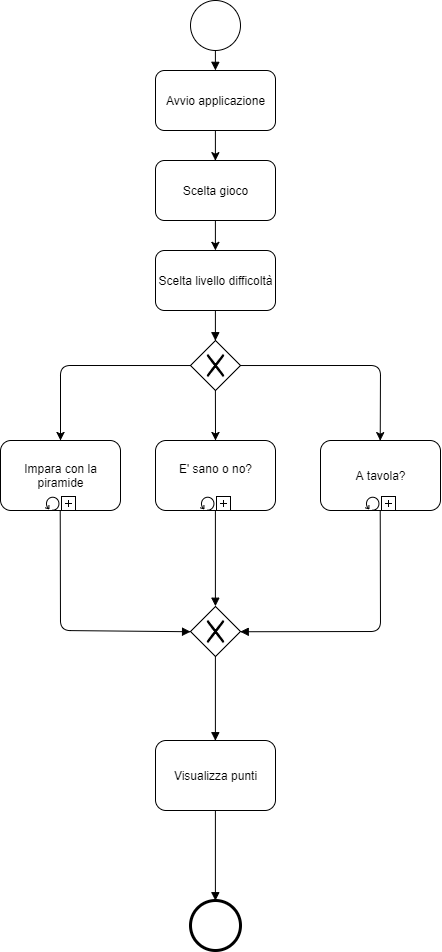
\includegraphics[scale=0.6]{Images/Flussogenerico}
\caption{Diagramma di flusso generale}
\label{fig:Diagramma di flusso generale}
\end{figure}
\clearpage

\begin{figure}[htbp]
\centering
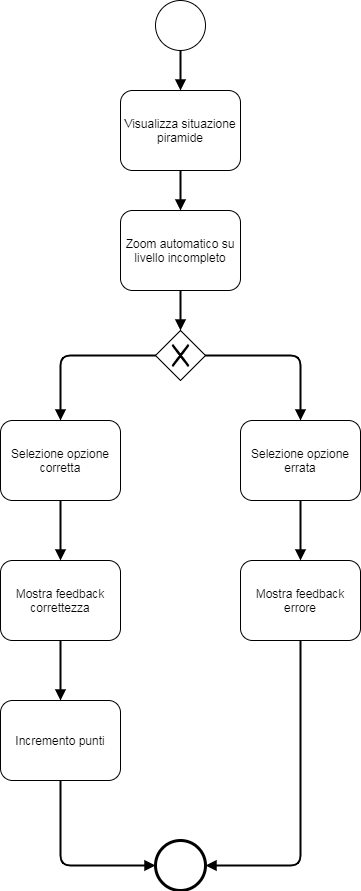
\includegraphics[scale=0.6]{Images/Flussopiramide}
\caption{Diagramma di flusso del gioco "Impara con la piramide"}
\label{fig:Diagramma di flusso del gioco "Impara con la piramide"}
\end{figure}
\clearpage

\begin{figure}[htbp]
\centering
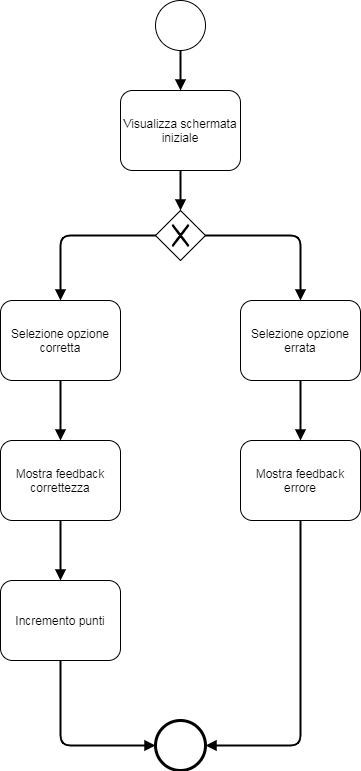
\includegraphics[scale=0.7]{Images/Flusso23}
\caption{Diagramma di flusso dei giochi "E' sano o no?" e "A tavola!"}
\label{fig:Diagramma di flusso dei giochi "E' sano o no?" e "A tavola!"}
\end{figure}
\clearpage

\subsection{Scenari} \label{scenari}
Di seguito vengono riportati tre scenari a rappresentazione dei giochi che si possono fare con \acs{gea}, sono tutti e tre di tipo testuale.
\subsubsection{Scenario 1}
Maria, terapista di un centro terapeutico per persone con disabilità, si trova nel suo studio pronta ad accogliere Emanuele, bimbo affetto da \acs{ndd}, per proseguire il loro percorso di educazione alimentare. Durante questa fase del laboratorio Maria decide di far uso di \acs{gea}, gioco di realtà virtuale per l'educazione alimentare, partendo da un livello basso di difficoltà. All'arrivo del bambino essa dunque avvia l'applicazione sopracitata e grazie al touchscreen seleziona il gioco "Impara con la piramide" perchè ha notato che Emanuele ha difficoltà nell'imparare quali alimenti si trovano in ogni specifico livello della piramide alimentare. Seleziona poi il livello "Facile" tra quelli possibili presentati e inserisce lo smartphone nel visore che il bambino va ad indossare. Il gioco mostra ad Emanuele prima l'intera piramide, una freccetta che punta uno specifico livello dando tre possibili scelte di completamento. Il bambino effettua con lo sguardo la sua scelta che risulta essere corretta per cui appare la mascotte GEA col viso sorridente a conferma.
\subsubsection{Scenario 2}
Alessia, bambina con disabilità, si sta recando con la mamma presso il centro terapeutico in cui è in cura piena di gioia perchè è Venerdì e quindi sa che farà laboratorio di alimentazione interattivo usando un gioco chiamato \acs{gea}. Una volta arrivata indossa, come ormai ben sa, il visore passatole dalla sua terapista che aveva precedentemente selezionato il gioco "E' sano o no?" perchè Alessia pasticcia un po' troppo nella sua alimentazione. La schermata che le appare mostra nella parte sinistra due pietanze differenti e sulla parte destra una pattumiera, lo scopo del gioco è quello di "buttare", trascinandolo con lo sguardo, nella pattumiera il piatto ritenuto cibo "spazzatura". Alessia con lo sguardo butta purtroppo il cibo errato e le appare la mascotte con il volto triste ad indicare la scelta erronea.
\clearpage
\subsubsection{Scenario 3}
Il papà di Alberto si reca insieme al figlio disabile presso il centro terapeutico perchè il bambino ha dei seri problemi di alimentazione ossia non riesce ad imparare quale pietanza sia adatta al pasto in considerazione. Sono ormai molte sedute che svolge con la sua terapista Dalila ed è arrivato il momento di rendere questo percorso di cura più interattivo grazie all'uso di \acs{gea}, un gioco per l'educazione alimentare. Dalila avvia l'applicazione, seleziona il gioco "A tavola!", seleziona la difficoltà e fa indossare il visore ad Alberto. Davanti agli occhi del bambino appare l'immagine di un bel piatto di pasta fumante con sotto le quattro opzioni: colazione, pranzo, merenda e cena. Il bambino preso da entusiasmo esclama ad alta voce cena e con lo sguardo punta la casella corrispondente: appare così la mascotte del gioco con il volto sorridente a conferma della scelta effettuata.
\clearpage

\subsection{Design iniziale: Mockup}

Il mockup in \textbf{Figura \ref{fig:Impara con la piramide}} mostra la schermata che comparirà dopo aver scelto di giocare a "Impara con la piramide" e dopo aver selezionato il livello di difficoltà desiderato. La schermata che appare spiega molto brevemente quello che il bambino dovrà fare giocando e quindi l'obiettivo da raggiungere.\\
Il mockup in \textbf{Figura \ref{fig:Piramide}} mostra la schermata successiva a quella esplicativa per quanto riguarda il gioco "Impara con la piramide". Qui viene mostrata al bambino l'intera piramide alimentare che il bambino dovrà via via completare durante il gioco.\\
Il mockup in \textbf{Figura \ref{fig:Piramide proseguimento}} viene presentata dopo aver mostrato l'intera piramide. Qui un puntatore indicherà un preciso livello della piramide alimentare che deve essere completato e si mostrano al bambino tre alimenti tra cui dover scegliere per effettuare il corretto completamento.\\
Il mockup in \textbf{Figura \ref{fig:E' sano o no?}} mostra la schermata che comparirà dopo aver scelto di giocare a "E' sano o no?" e dopo aver selezionato il livello di difficoltà desiderato. La schermata che appare spiega molto brevemente quello che il bambino dovrà fare giocando e quindi l'obiettivo da raggiungere.\\
Il mockup in \textbf{Figura \ref{fig:Schermata "E' sano o no?"}} mostra la schermata successiva a quella esplicativa per quanto riguarda il gioco "E' sano o no?". Qui vengono mostrati al bambino due pietanze tra le quali deve scegliere il cibo "spazzatura" e "buttarlo" con lo sguardo nella pattumiera presente sulla destra della schermata.\\
Il mockup in \textbf{Figura \ref{fig:Scelta "E' sano o no?"}} mostra la schermata relativa al compimento di una scelta: nel caso presentato la scelta è errata.\\
Il mockup in \textbf{Figura \ref{fig:A tavola!}} mostra la schermata che comparirà dopo aver scelto di giocare a "A tavola!" e dopo aver selezionato il livello di difficoltà desiderato. La schermata che appare spiega molto brevemente quello che il bambino dovrà fare giocando e quindi l'obiettivo da raggiungere.\\
Il mockup in \textbf{Figura \ref{fig:Schermata "A tavola!"}} mostra la schermata successiva a quella esplicativa per quanto riguarda il gioco "A tavola!". Qui vengono mostrati al bambino una pietanza e due possibili pasti del giorno: egli deve scegliere qual è il pasto più adatto per consumare quella pietanza. Il gioco si può presentare anche nella forma opposta ossia scegliere fra due piatti quale sia più adatto per il pasto indicato.\\
Il mockup in \textbf{Figura \ref{fig:Scelta "A tavola!"}} mostra la schermata relativa al compimento di una scelta: nel caso presentato la scelta è corretta.

\begin{figure*}
 \begin{minipage}[c]{\columnwidth}
   \centering
   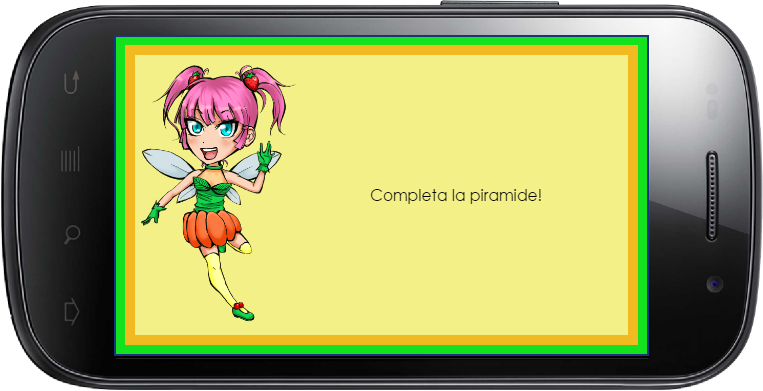
\includegraphics[width=8cm]{Images/Mockup/gioco1}
   \caption{Impara con la piramide mockup}
   \label{fig:Impara con la piramide}
 \end{minipage}
 \ \hspace{8mm} \hspace{8mm} \\\
 
 \begin{minipage}[c]{\columnwidth}
  \centering
   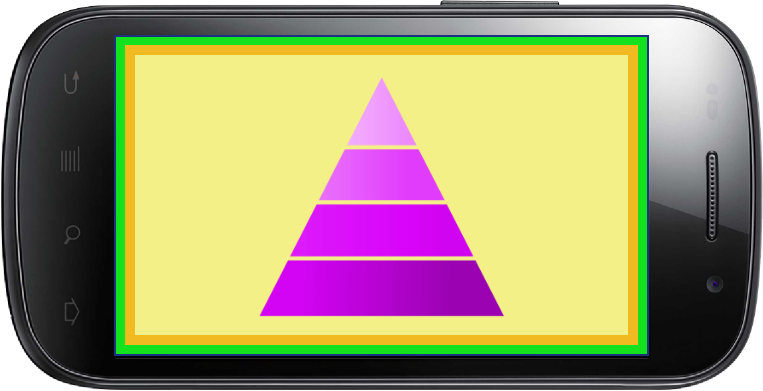
\includegraphics[width=8cm]{Images/Mockup/piramide}
   \caption{Piramide mockup}
   \label{fig:Piramide}
 \end{minipage}
 \ \hspace{8mm} \hspace{8mm} \\\
 
 \begin{minipage}[c]{\columnwidth}
  \centering
   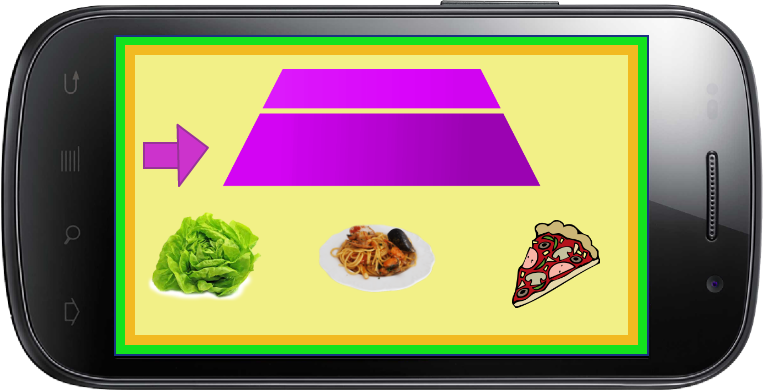
\includegraphics[width=8cm]{Images/Mockup/piramide2}
   \caption{Piramide proseguimento mockup}
   \label{fig:Piramide proseguimento}
 \end{minipage}
\end{figure*}
\clearpage

\begin{figure*}
 \begin{minipage}[c]{\columnwidth}
   \centering
   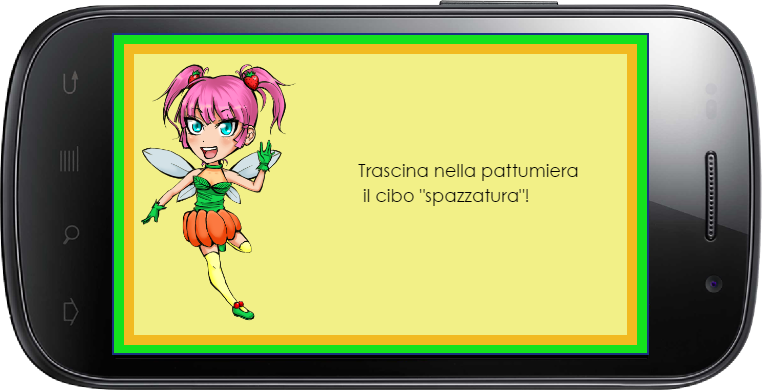
\includegraphics[width=8cm]{Images/Mockup/gioco2}
   \caption{E' sano o no? mockup}
   \label{fig:E' sano o no?}
 \end{minipage}
 \ \hspace{8mm} \hspace{8mm} \\\
 
 \begin{minipage}[c]{\columnwidth}
  \centering
   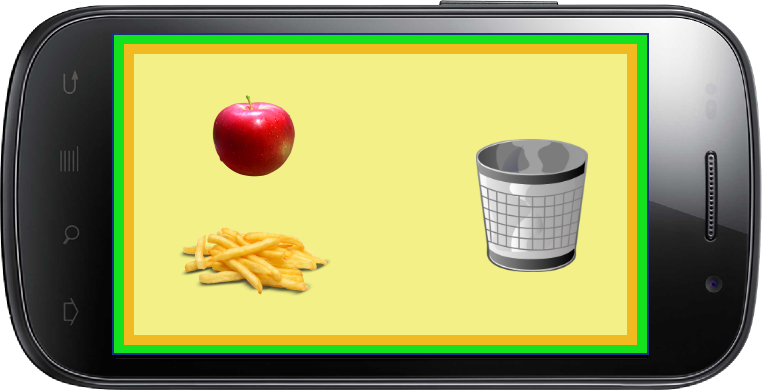
\includegraphics[width=8cm]{Images/Mockup/sano}
   \caption{Schermata "E' sano o no?" mockup}
   \label{fig:Schermata "E' sano o no?"}
 \end{minipage}
 \ \hspace{8mm} \hspace{8mm} \\\
 
 \begin{minipage}[c]{\columnwidth}
  \centering
   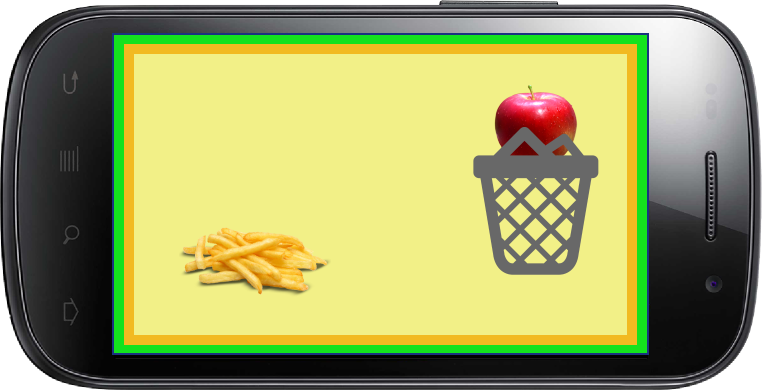
\includegraphics[width=8cm]{Images/Mockup/sanoscelta}
   \caption{Scelta cibo "spazzatura" mockup}
   \label{fig:Scelta "E' sano o no?"}
 \end{minipage}
\end{figure*}
\clearpage

\begin{figure*}
 \begin{minipage}[c]{\columnwidth}
   \centering
   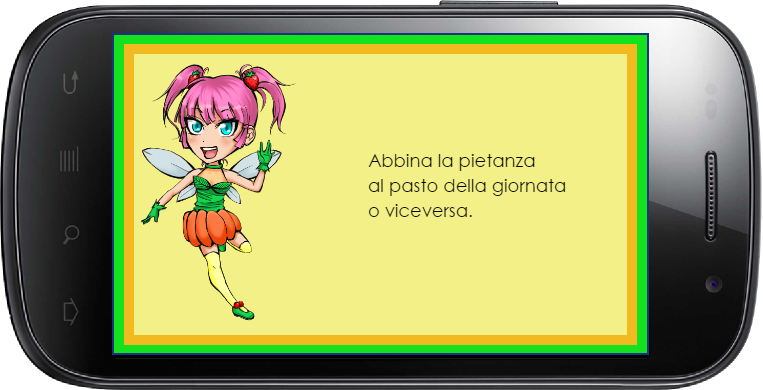
\includegraphics[width=8cm]{Images/Mockup/gioco3}
   \caption{A tavola! mockup}
   \label{fig:A tavola!}
 \end{minipage}
 \ \hspace{8mm} \hspace{8mm} \\\
 
 \begin{minipage}[c]{\columnwidth}
  \centering
   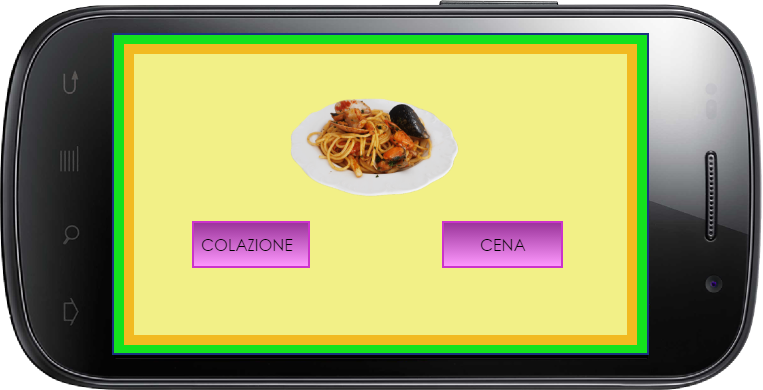
\includegraphics[width=8cm]{Images/Mockup/atavola}
   \caption{Schermata "A tavola!" mockup}
   \label{fig:Schermata "A tavola!"}
 \end{minipage}
 \ \hspace{8mm} \hspace{8mm} \\\
 
 \begin{minipage}[c]{\columnwidth}
  \centering
   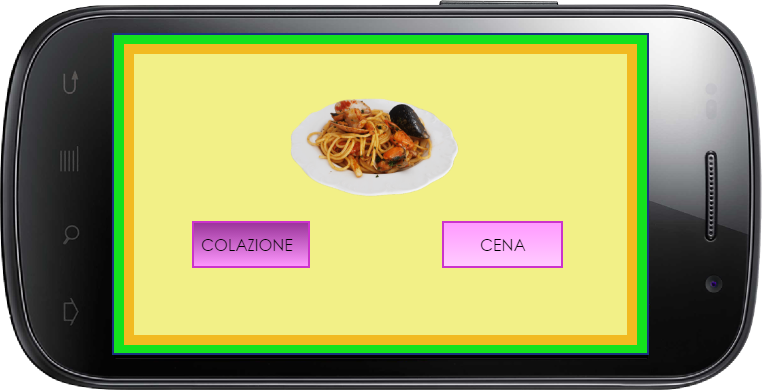
\includegraphics[width=8cm]{Images/Mockup/atavolascelta}
   \caption{Scelta pasto mockup}
   \label{fig:Scelta "A tavola!"}
 \end{minipage}
\end{figure*}
\clearpage


\subsection{Design attuale}
Di seguito vengono riportati alcuni screenshot riguardati il design attuale di \acs{gea}.\\
Le due immagini qui riportate si riferiscono alla schermata di home di \acs{gea} in landascape e in portscape. Qui si può effettuare la scelta riguardante la tipologia di gioco che si vuole effettuare.

\begin{center}
\begin{minipage}[c]{.40\textwidth}
\centering
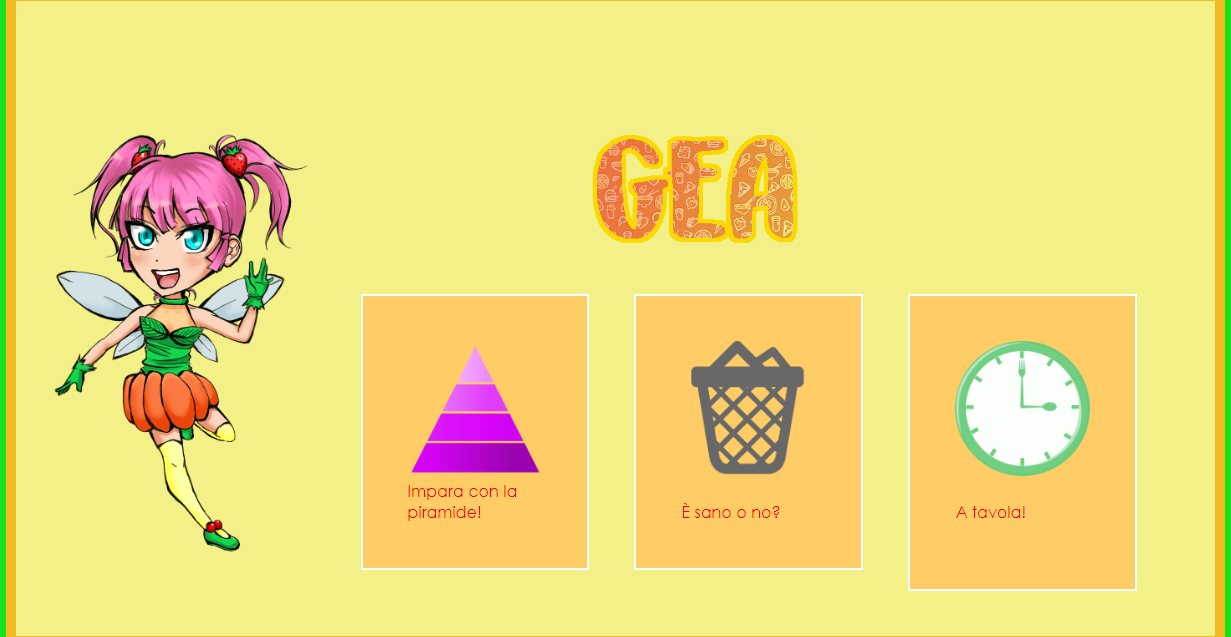
\includegraphics[width=.70\textwidth]{Images/Design/Game}\\
\vspace{10px}
\emph{Schermata iniziale pc}\bigskip
\end{minipage}
\hspace{10mm}
\begin{minipage}[c]{.40\textwidth}
\centering
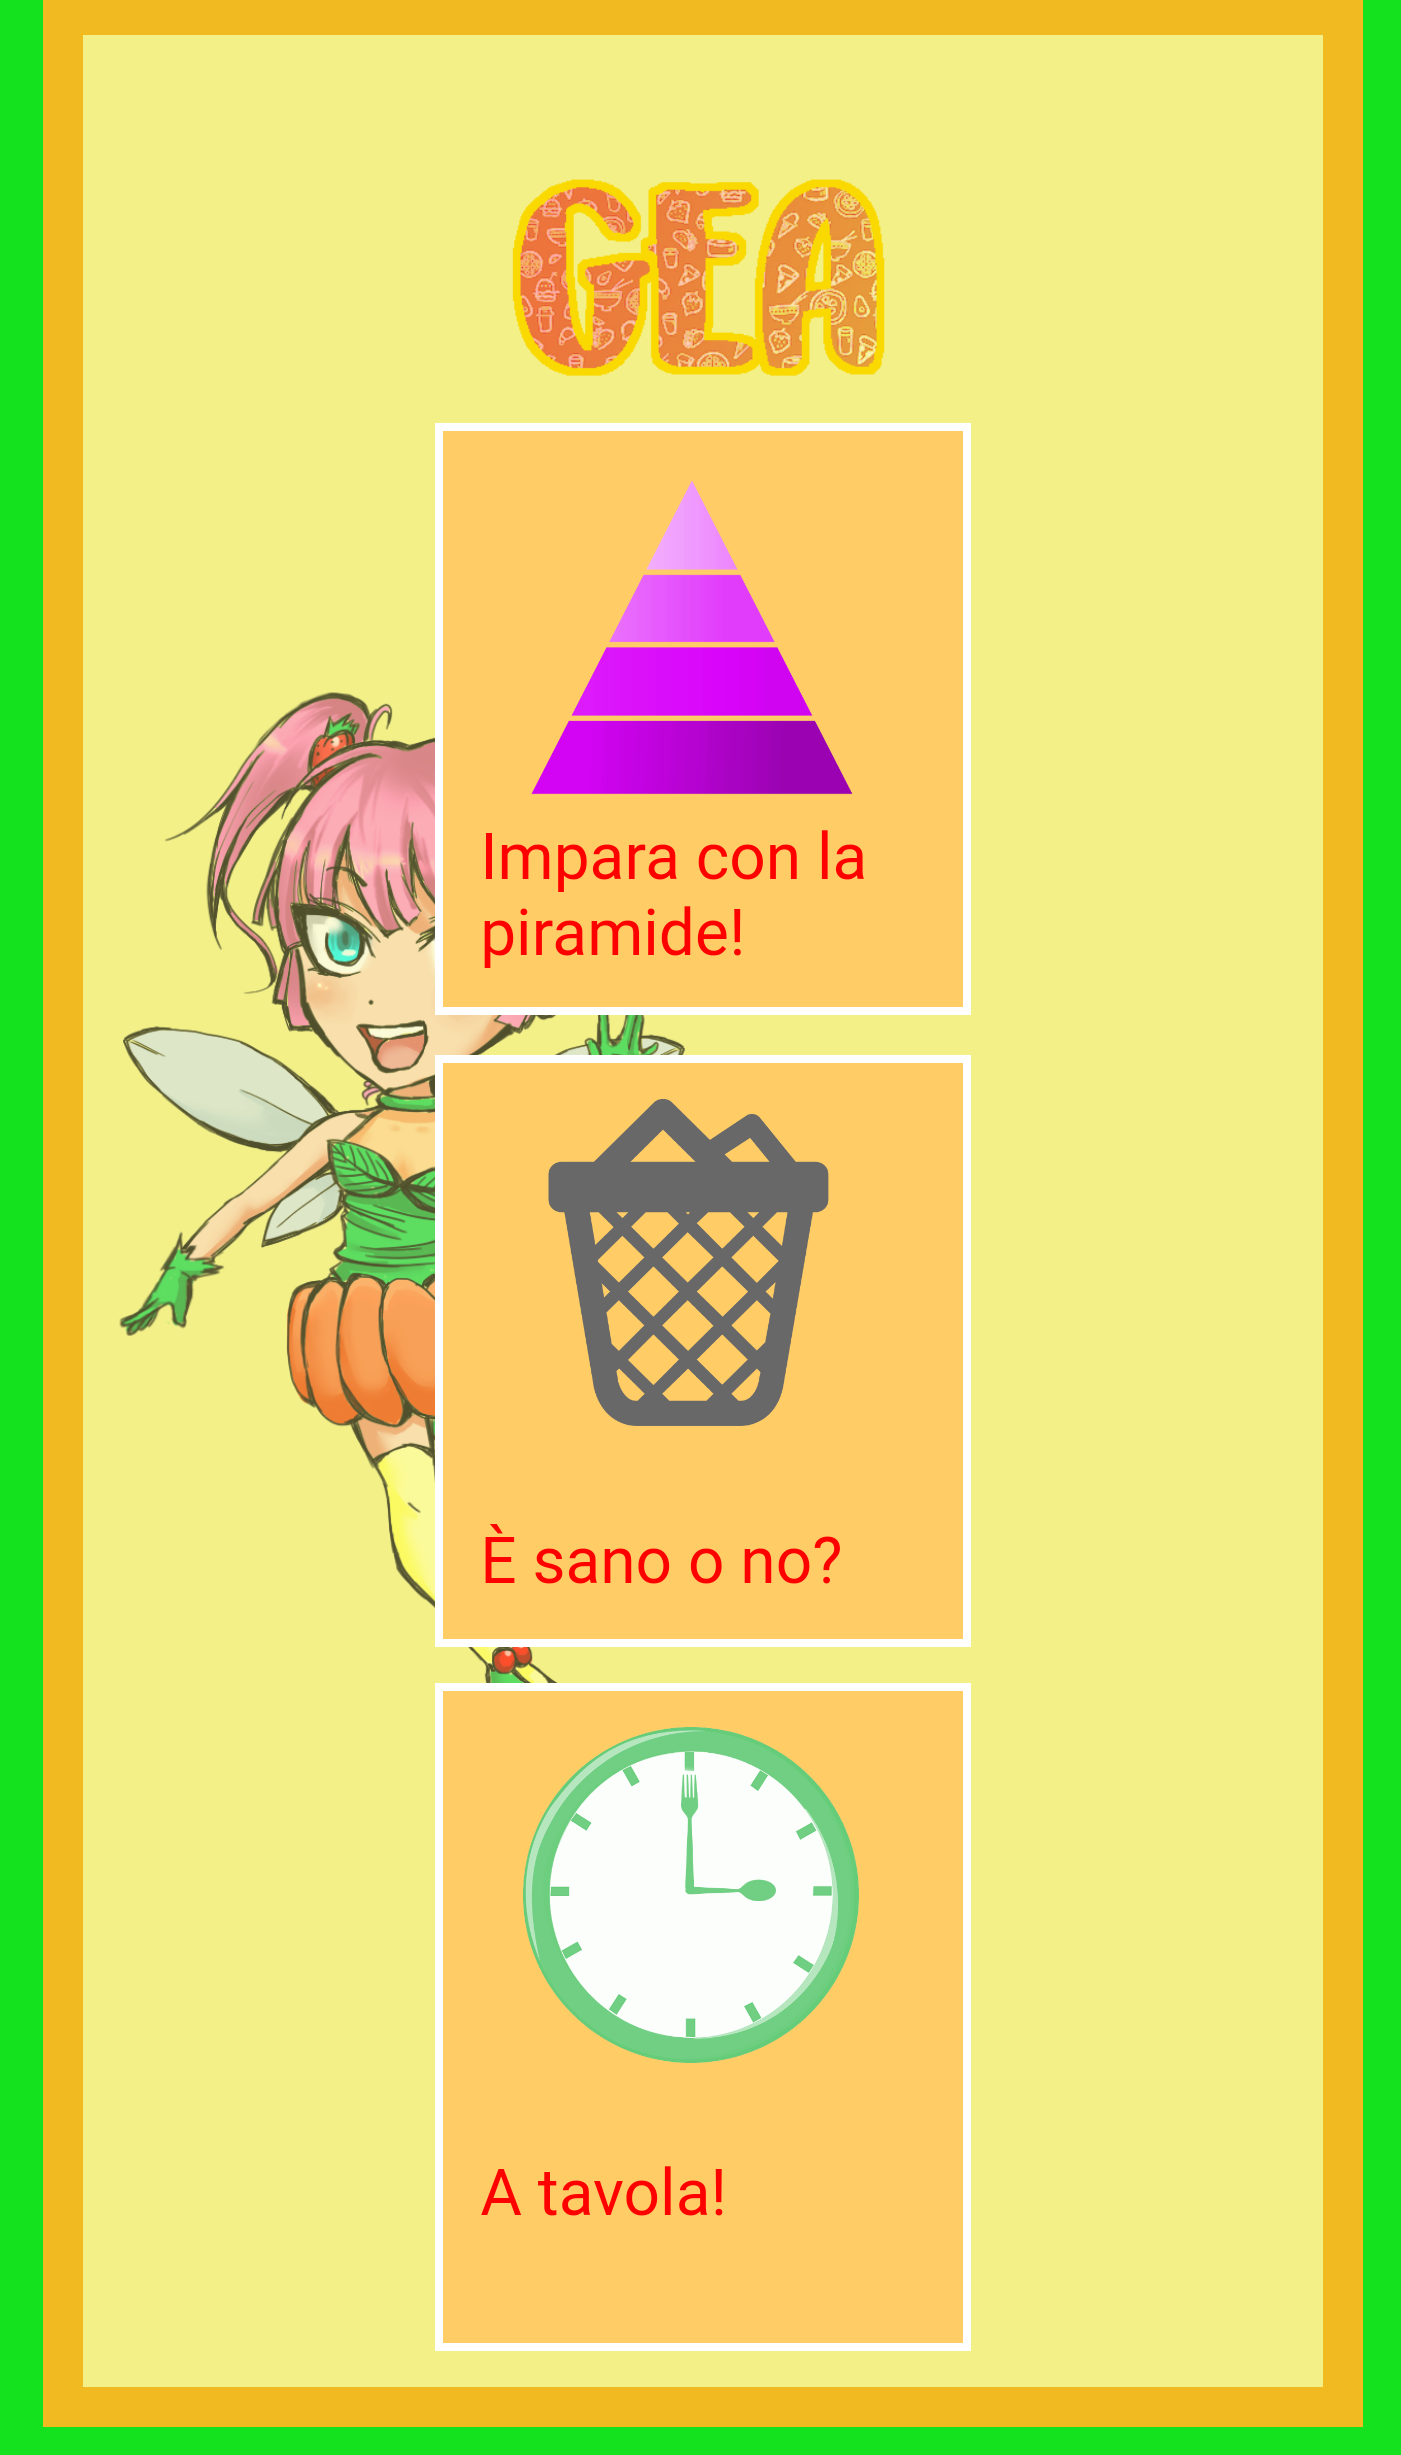
\includegraphics[width=.70\textwidth]{Images/Design/Homesmartphone}\\
\vspace{10px}
\emph{Schermata iniziale smartphone}\bigskip
\end{minipage}
\end{center}

La prossima immagine si riferisce invece alla schermata successiva alla scelta di gioco che riguarda la possibilità di selezionare il livello di difficoltà desiderato oppure tornare alla schermata precedente.
\begin{figure}[htbp]
\centering
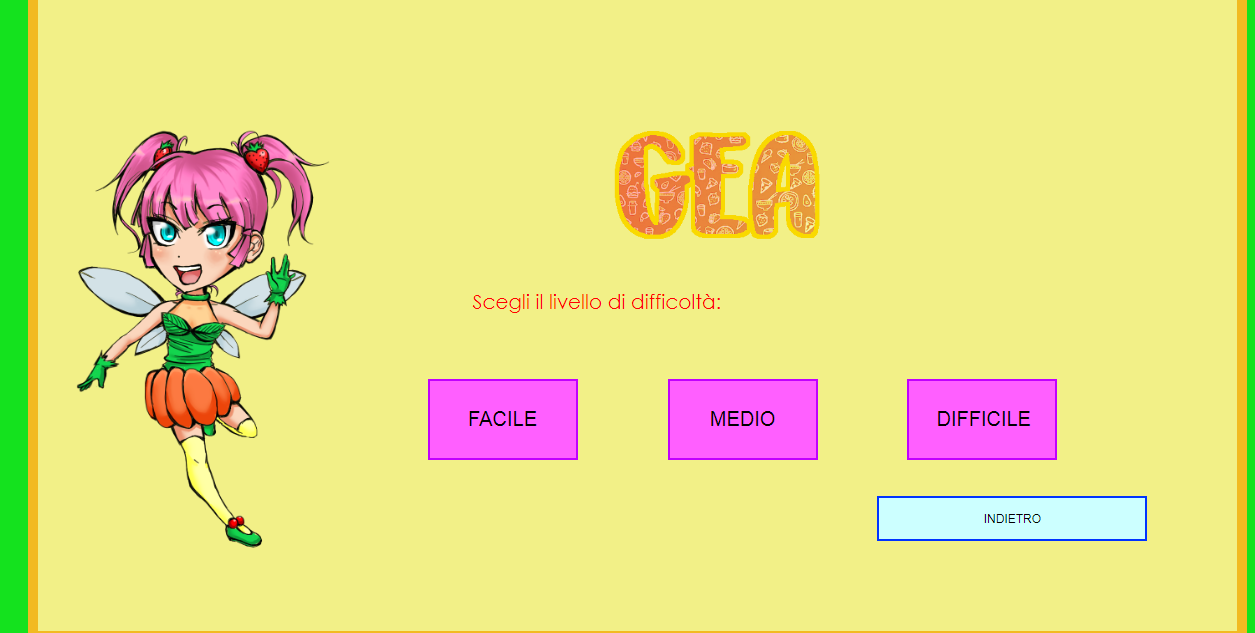
\includegraphics[width=.70\textwidth]{Images/Design/Level}\\
\vspace{10px}
\emph{Scelta livello di difficoltà}\bigskip
\end{figure}

I tre screenshot di seguito si riferiscono rispettivamente all'avvio dei tre giochi.
\begin{center}
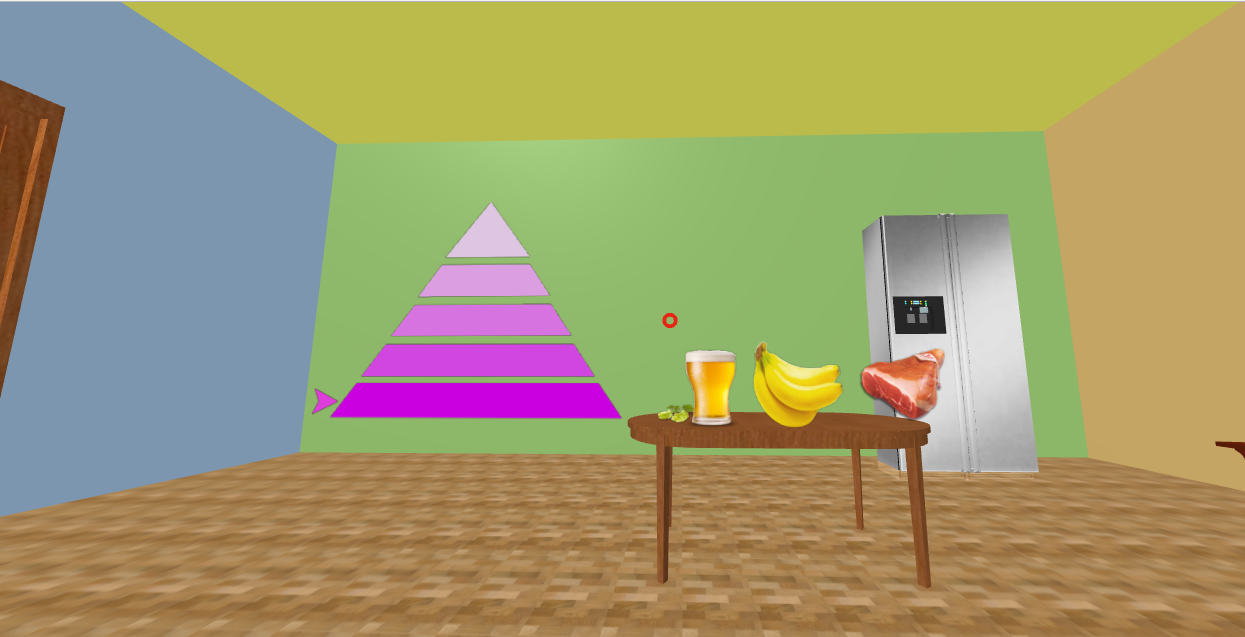
\includegraphics[width=.70\textwidth]{Images/Design/pyramid}\\
\vspace{5px}
\emph{Gioco 1: Impara con la piramide!}\bigskip
\end{center}
\begin{center}
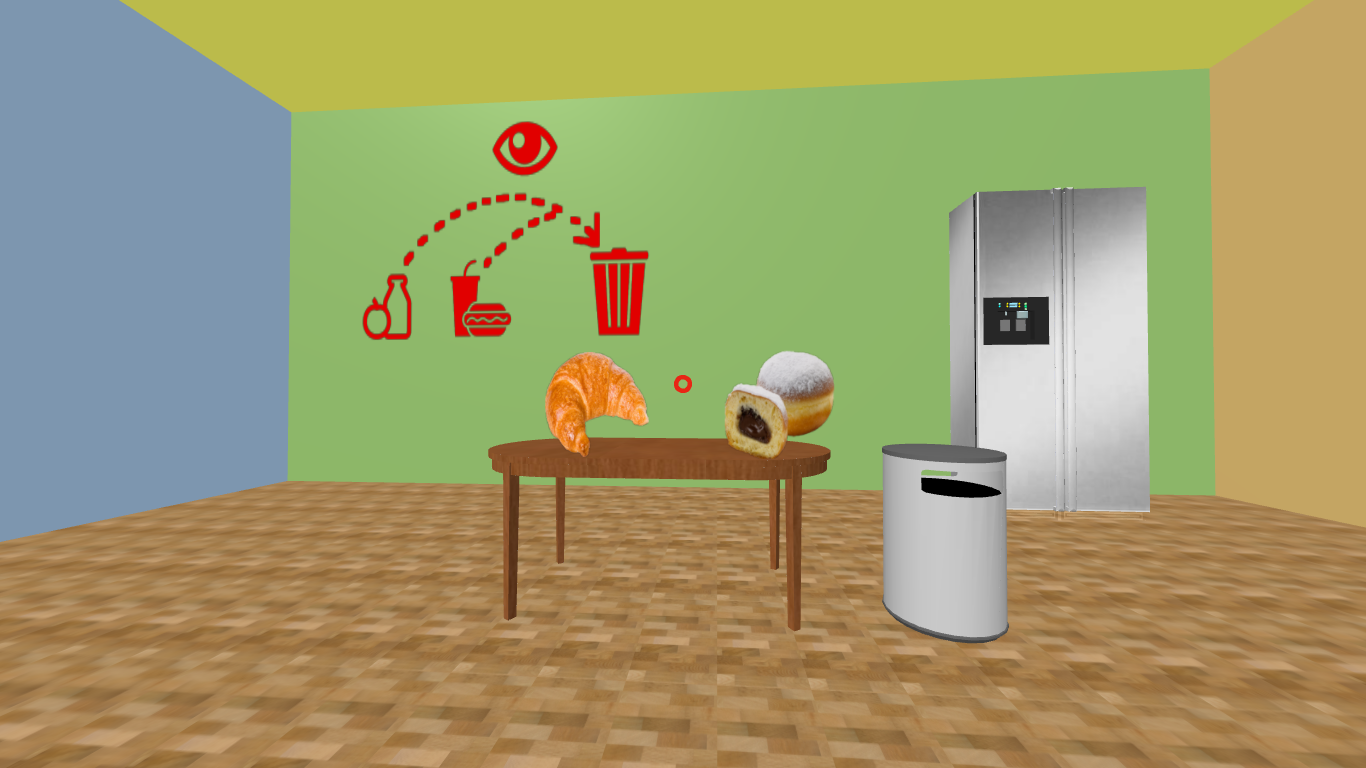
\includegraphics[width=.70\textwidth]{Images/Design/Healthy}\\
\vspace{5px}
\emph{Gioco 2: E' sano o no?}\bigskip
\end{center}
\begin{center}
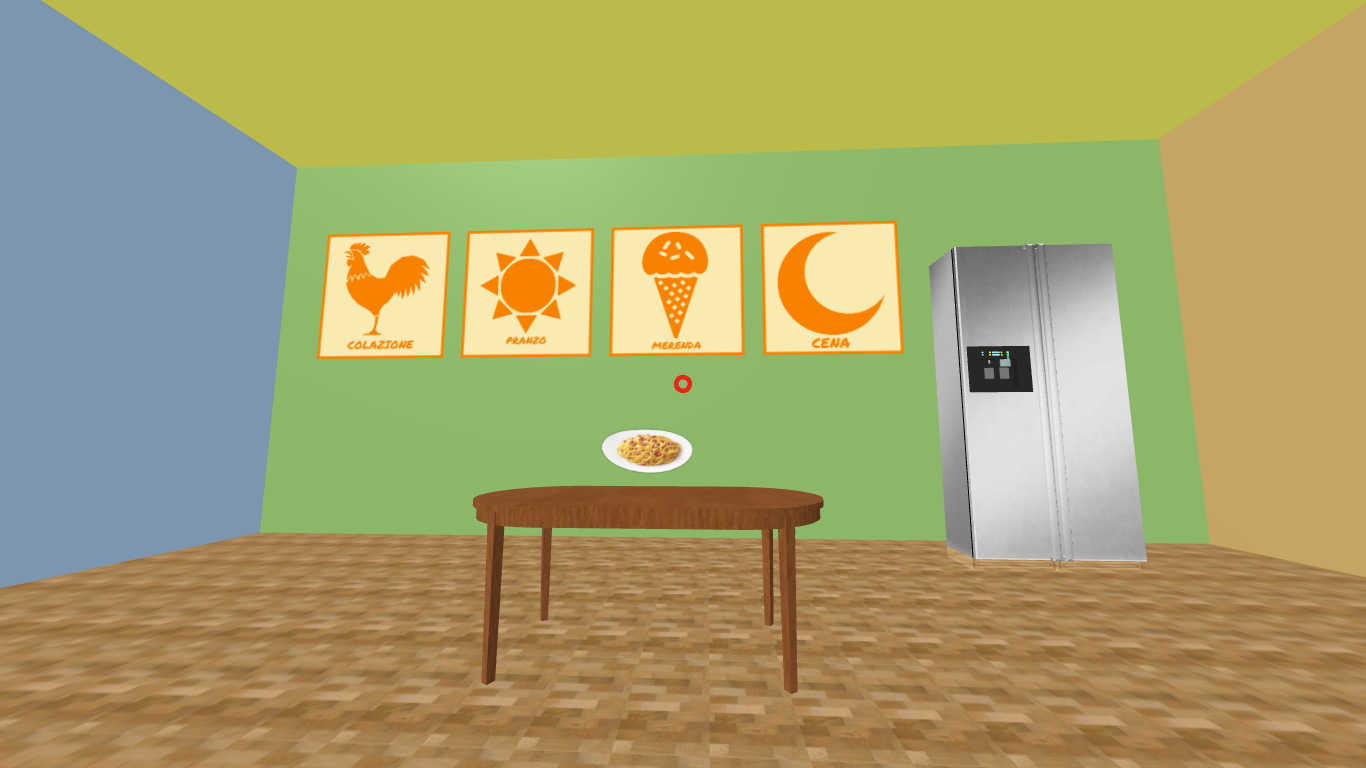
\includegraphics[width=.70\textwidth]{Images/Design/Eat}\\
\vspace{5px}
\emph{Gioco 3: A tavola!}\bigskip
\end{center}
\clearpage

Le due immagini successive rappresentano i feedback mostrati dopo che una scelta viene effettuata: la mascotte del gioco apparirà con volto felice in caso di risposta corretta e con volto triste nel caso di risposta errata. Per quanto riguarda il primo gioco si avrà inoltre il rispettivo livello della piramide che si colora di verde o rosso a ricordare durante il resto della partita le scelte giuste o sbagliate.
\begin{center}
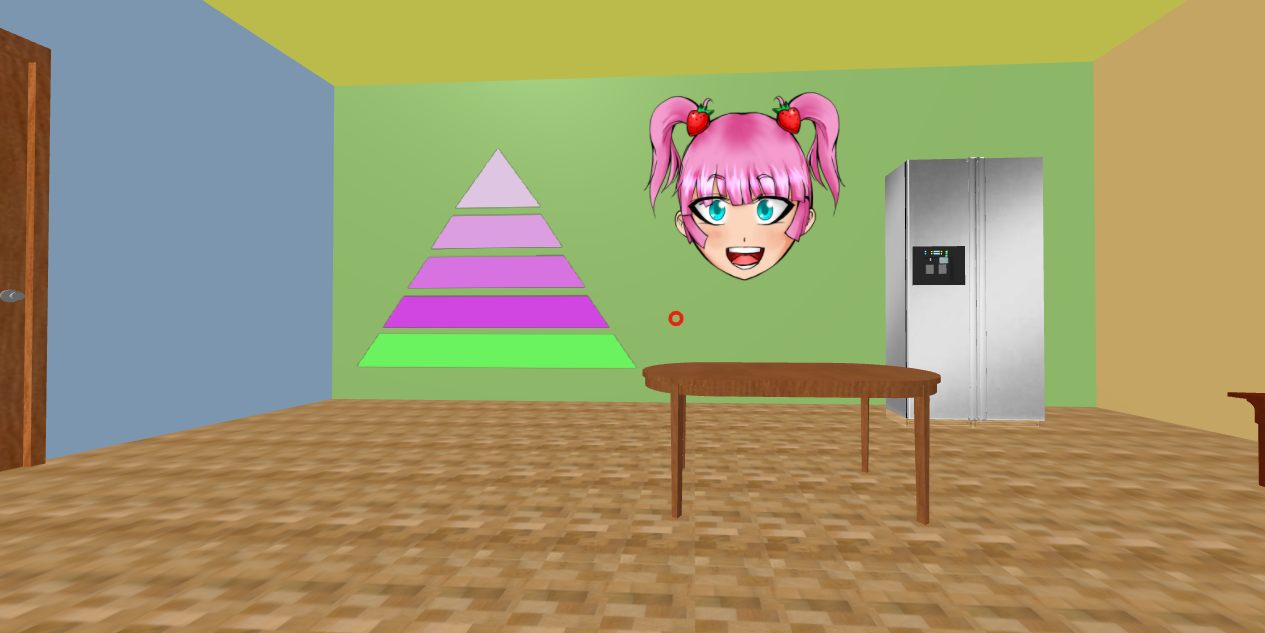
\includegraphics[width=.70\textwidth]{Images/Design/Correct}\\
\vspace{5px}
\emph{Feedback risposta corretta}\bigskip
\end{center}
\begin{center}
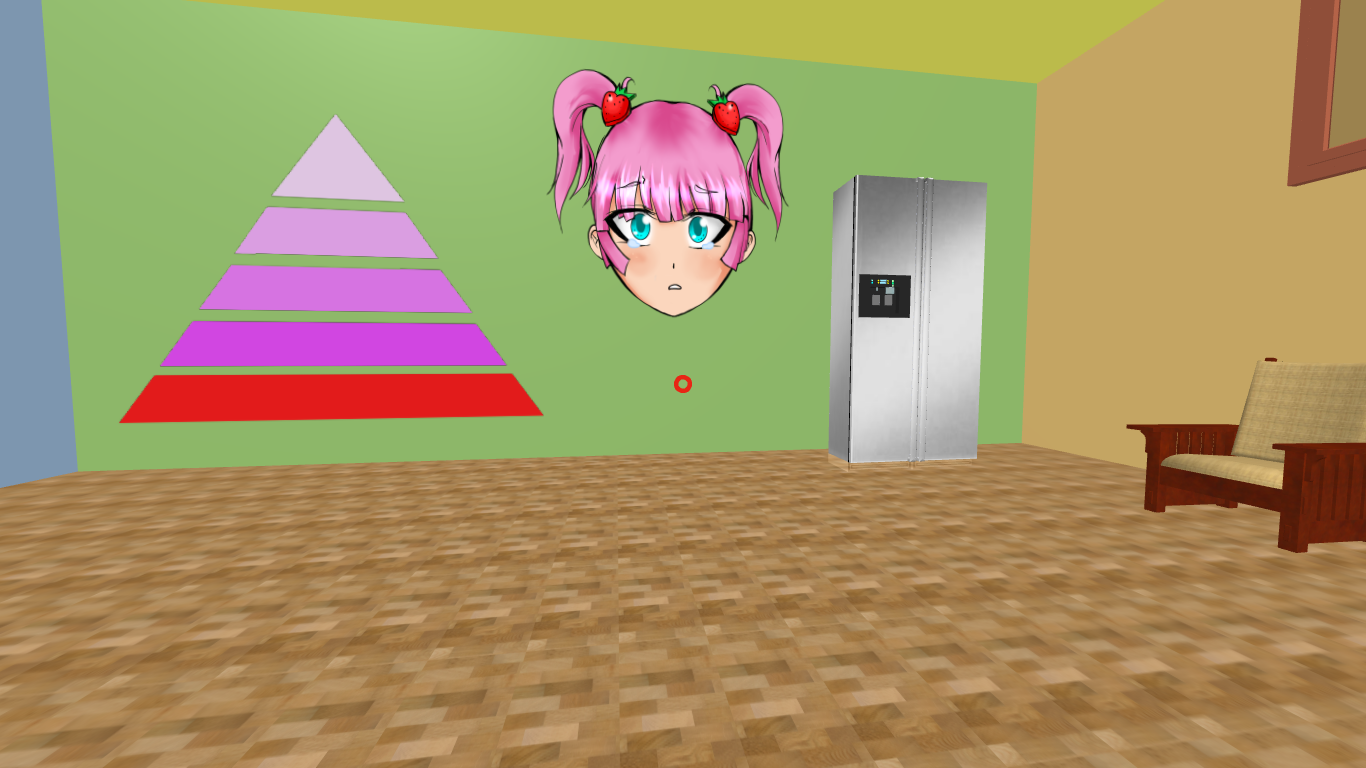
\includegraphics[width=.70\textwidth]{Images/Design/Wrong}\\
\vspace{5px}
\emph{Feedback risposta errata}\bigskip
\end{center}